\documentclass[tikz,border=10pt]{standalone}
\usepackage{tikz}
\usepackage{amsmath}
\usetikzlibrary{patterns, arrows.meta, decorations.pathreplacing, calc, positioning}

\begin{document}
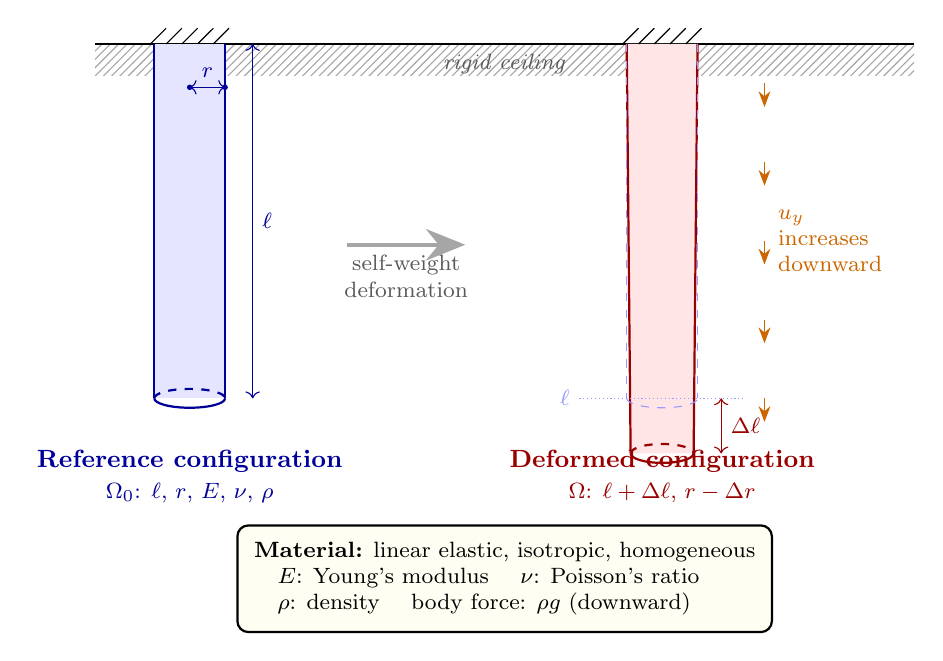
\begin{tikzpicture}[scale=1.0, every node/.style={font=\small}]

    % =========================================================
    % CEILING (hatched region)
    % =========================================================
    % Ceiling wall fill
    \fill[pattern=north east lines, pattern color=gray!70] 
        (-1.2, 0) rectangle (9.2, -0.4);
    \draw[thick] (-1.2, 0) -- (9.2, 0);
    \node[font=\footnotesize, gray!70!black] at (4.0, -0.25) 
        {\textit{rigid ceiling}};
    
    % =========================================================
    % LEFT: Undeformed reference configuration
    % =========================================================
    % Bar dimensions (schematic): radius r (schematic), length l
    \def\rbar{0.45}
    \def\lbar{4.5}
    
    % Undeformed bar (left, at x=0)
    \coordinate (topL) at (0, 0);
    \coordinate (botL) at (0, -\lbar);
    
    % Bar sides (rectangle approximating the cylindrical bar in 2D projection)
    \fill[blue!10] (-\rbar, 0) rectangle (\rbar, -\lbar);
    \draw[thick, blue!60!black] (-\rbar, 0) -- (-\rbar, -\lbar);
    \draw[thick, blue!60!black] (\rbar, 0) -- (\rbar, -\lbar);
    % Bottom (slightly elliptical to suggest circular cross-section)
    \draw[thick, blue!60!black] (-\rbar, -\lbar) 
        arc (180:360:{\rbar} and 0.12);
    \draw[thick, blue!60!black, dashed] (-\rbar, -\lbar) 
        arc (180:0:{\rbar} and 0.12);
    
    % Fixed support symbol (hatch marks on top)
    \foreach \x in {-0.4, -0.2, 0, 0.2, 0.4} {
        \draw[thin] (\x-0.1, 0) -- (\x+0.1, 0.2);
    }
    
    % Radius annotation at top
    \draw[<->, thin, blue!60!black] (0, -0.55) -- (\rbar, -0.55);
    \node[blue!60!black, font=\footnotesize, above] at (\rbar/2, -0.55) {$r$};
    \fill[blue!60!black] (0, -0.55) circle (1pt);
    \fill[blue!60!black] (\rbar, -0.55) circle (1pt);
    
    % Length annotation
    \draw[<->, thin, blue!60!black] (\rbar+0.35, 0) -- (\rbar+0.35, -\lbar);
    \node[blue!60!black, font=\footnotesize, right] 
        at (\rbar+0.35, -\lbar/2) {$\ell$};
    
    % Label
    \node[font=\small\bfseries, blue!60!black] at (0, -5.3) 
        {Reference configuration};
    \node[font=\footnotesize, blue!60!black] at (0, -5.7) 
        {$\Omega_0$: $\ell$, $r$, $E$, $\nu$, $\rho$};

    % =========================================================
    % MIDDLE: Arrow showing deformation
    % =========================================================
    \draw[-{Stealth[length=5mm, width=4mm]}, ultra thick, gray!70] 
        (2.0, -\lbar/2 - 0.3) -- (3.5, -\lbar/2 - 0.3);
    \node[gray!70!black, font=\footnotesize, align=center] 
        at (2.75, -\lbar/2 - 0.7) {self-weight\\deformation};

    % =========================================================
    % RIGHT: Deformed configuration
    % =========================================================
    \def\xR{6.0}   % Right panel origin
    % Deformed shape: stretch with slight lateral contraction (Poisson effect)
    % Vertical elongation under self-weight: nonuniform (max at bottom)
    % We draw a stretched bar with slight taper due to Poisson effect
    
    \def\rcap{0.40}   % Slightly smaller at the deformed state
    \def\lcap{5.2}    % Slightly longer (stretched)
    
    % Deformed bar fill (slightly tapered to hint at Poisson contraction)
    \fill[red!10] 
        (\xR-\rbar, 0) -- 
        (\xR-\rcap, -\lcap) -- 
        (\xR+\rcap, -\lcap) -- 
        (\xR+\rbar, 0) -- cycle;
    
    % Deformed bar edges
    \draw[thick, red!60!black] (\xR-\rbar, 0) -- (\xR-\rcap, -\lcap);
    \draw[thick, red!60!black] (\xR+\rbar, 0) -- (\xR+\rcap, -\lcap);
    \draw[thick, red!60!black] (\xR-\rcap, -\lcap) 
        arc (180:360:{\rcap} and 0.12);
    \draw[thick, red!60!black, dashed] (\xR-\rcap, -\lcap) 
        arc (180:0:{\rcap} and 0.12);
    
    % Original position (ghost) for comparison
    \draw[thin, blue!40, dashed] (\xR-\rbar, 0) -- (\xR-\rbar, -\lbar);
    \draw[thin, blue!40, dashed] (\xR+\rbar, 0) -- (\xR+\rbar, -\lbar);
    \draw[thin, blue!40, dashed] (\xR-\rbar, -\lbar) 
        arc (180:360:{\rbar} and 0.12);
    
    % Fixed support
    \foreach \x in {\xR-0.4, \xR-0.2, \xR, \xR+0.2, \xR+0.4} {
        \draw[thin] (\x-0.1, 0) -- (\x+0.1, 0.2);
    }
    
    % Elongation annotation (Δℓ)
    \draw[<->, thin, red!60!black] (\xR+\rcap+0.35, -\lbar) -- 
        (\xR+\rcap+0.35, -\lcap);
    \node[red!60!black, font=\footnotesize, right] 
        at (\xR+\rcap+0.35, {-(0.5*\lbar+0.5*\lcap)}) {$\Delta\ell$};
    
    % Reference length indicator
    \draw[thin, blue!40, densely dotted] (\xR-\rbar-0.6, -\lbar) -- 
        (\xR+\rbar+0.6, -\lbar);
    \node[blue!40, font=\footnotesize, left] 
        at (\xR-\rbar-0.6, -\lbar) {$\ell$};
    
    % Label
    \node[font=\small\bfseries, red!60!black] at (\xR, -5.3) 
        {Deformed configuration};
    \node[font=\footnotesize, red!60!black] at (\xR, -5.7) 
        {$\Omega$: $\ell + \Delta\ell$, $r - \Delta r$};
    
    % =========================================================
    % Displacement field annotation (u_y)
    % =========================================================
    % Small arrows suggesting downward displacement gradient
    \foreach \y in {-0.5, -1.5, -2.5, -3.5, -4.5} {
        \draw[-{Stealth[length=2mm]}, thin, orange!80!black] 
            (\xR+\rcap+0.9, \y) -- (\xR+\rcap+0.9, \y-0.3);
    }
    \node[orange!80!black, font=\footnotesize, right, align=left] 
        at (\xR+\rcap+0.95, -2.5) {$u_y$\\increases\\downward};

    % =========================================================
    % Material parameters box
    % =========================================================
    \node[draw, rounded corners, fill=yellow!5, thick, 
          font=\footnotesize, inner sep=6pt, align=left,
          anchor=north] at (4.0, -6.1) {
        \textbf{Material:} linear elastic, isotropic, homogeneous \\
        \quad $E$: Young's modulus \quad $\nu$: Poisson's ratio \\
        \quad $\rho$: density \quad body force: $\rho g$ (downward)
    };

\end{tikzpicture}
\end{document}
